\documentclass[12pt,letterpaper]{article}

\def\myauthor{Juno~Woods}
\def\mytitle{jow-vita}
\def\myemail{juno@translunar.io}
\def\myweb{translunar}
\def\myphone{703-801-2625}
\def\mykeywords{
  juno woods,
  juno september woods,
  juno s woods,
  resume, 
  curriculum, 
  vita, 
  curriculum vita, 
  cv, 
  woods,
  linear covariance analysis,
  lincov,
  ekf,
  extended kalman filter,
  kalman filter,
  candidate optimal groups,
  cog,
  state estimation,
  gn\&c,
  navigation,
  control,
  guidance,
  powered explicit guidance,
  orbit determination,
  batch least squares,
  batch estimator,
  sequential filter,
  navigation filter,
  LunaNet,
  trajectory optimization,
  mission design,
  export control,
  open source,
  patched conic,
  cr3bp,
  trajectory design,
  space policy,
  bioinformatics,
  systems biology,
  synthetic biology,
  personalized medicine,
  computational biology
  automation,
  control systems,
  PID controllers,
  finite state automata,
  state machines,
  programmable logic controllers,
  zeromq,
  0mq
}

\setlength\parindent{0pt}

\newenvironment{itemize*}%
{\begin{itemize}%
  \setlength{\itemsep}{0pt}}%
{\end{itemize}}

\usepackage{graphicx}
\usepackage{wrapfig}
\usepackage{pgfplots}
\usepackage{amsmath}
\usepackage{textcomp}
\usepackage{url}
\usepackage{fancyhdr}
\usepackage{amssymb}
%\headheight 15ptz
\usepackage{lastpage}
%\usepackage{ocgtools}
\usepackage{enumitem}
\setlist{nolistsep,leftmargin=0.15in}
\usepackage[log-declarations=false]{xparse}
%\usepackage{mathdesign}
%\usepackage[no-math]{fontspec}
\usepackage{microtype}
\usepackage{bold-extra}
\usepackage[margin=1.125in,top=1.375in,right=1in,left=2in]{geometry}
\usepackage[strict]{changepage}
\usepackage[
  ocgcolorlinks,
  urlcolor={[rgb]{0,0,0.54}},
  unicode,
  plainpages=false,
  pdfpagelabels,
  pdftitle={\mytitle},
  pdfauthor={\myauthor},
  pdfkeywords={\mykeywords}
]{hyperref}
\usepackage{relsize}

% Use sans serif fonts in plot
\usepackage[eulergreek]{sansmath}
\pgfplotsset{
  every axis/.append style = {font=\sansmath\sffamily},
  %every axis label = {font=\sansmath\sffamily},
  %legend style = {font=\sansmath\sffamily},
  %tick label style = {font=\sansmath\sffamily},
  %every node style = {font=\sansmath\sffamily}
  }

% fix ocgcolor link breaking; thanks due to Benjamin Lerner (http://goo.gl/VZKR7M)
\makeatletter
\AtBeginDocument{%
  \newlength{\temp@x}%
  \newlength{\temp@y}%
  \newlength{\temp@w}%
  \newlength{\temp@h}%
  \def\my@coords#1#2#3#4{%
    \setlength{\temp@x}{#1}%
    \setlength{\temp@y}{#2}%
    \setlength{\temp@w}{#3}%
    \setlength{\temp@h}{#4}%
    \adjustlengths{}%
    \my@pdfliteral{\strip@pt\temp@x\space\strip@pt\temp@y\space\strip@pt\temp@w\space\strip@pt\temp@h\space re}}%
  \ifpdf
    \typeout{In PDF mode}%
    \def\my@pdfliteral#1{\pdfliteral page{#1}}% I don't know why % this command...
    \def\adjustlengths{}%
  \fi
  \ifxetex
    \def\my@pdfliteral #1{\special{pdf: literal direct #1}}% isn't equivalent to this one
    \def\adjustlengths{\setlength{\temp@h}{-\temp@h}\addtolength{\temp@y}{1in}\addtolength{\temp@x}{-1in}}%
  \fi%
  \def\Hy@colorlink#1{%
    \begingroup
      \ifHy@ocgcolorlinks
        \def\Hy@ocgcolor{#1}%
        \my@pdfliteral{q}%
        \my@pdfliteral{7 Tr}% Set text mode to clipping-only
      \else
        \HyColor@UseColor#1%
      \fi
  }%
  \def\Hy@endcolorlink{%
    \ifHy@ocgcolorlinks%
      \my@pdfliteral{/OC/OCPrint BDC}%
      \my@coords{0pt}{0pt}{\pdfpagewidth}{\pdfpageheight}%
      \my@pdfliteral{F}% Fill clipping path (the url's text) with current color
      \my@pdfliteral{EMC/OC/OCView BDC}%
      \begingroup%
        \expandafter\HyColor@UseColor\Hy@ocgcolor%
        \my@coords{0pt}{0pt}{\pdfpagewidth}{\pdfpageheight}%
        \my@pdfliteral{F}% Fill clipping path (the url's text) with \Hy@ocgcolor
      \endgroup%
      \my@pdfliteral{EMC}%
      \my@pdfliteral{0 Tr}% Reset text to normal mode
      \my@pdfliteral{Q}%
    \fi
    \endgroup
  }%
}
\makeatother
% end fixes


\newcommand{\Cpp}{\textsc{c}\nolinebreak[4]\hspace{-.05em}\raisebox{.4ex}{\relsize{-3}{\textbf{++}}}}
\newcommand{\Magickpp}{Magick\nolinebreak[4]\hspace{-.05em}\raisebox{.4ex}{\relsize{-3}{\textbf{++}}}}
\newcommand{\Star}{\textsc{Star-CCM\ensuremath{+}}}

\newcommand{\mhead}[1]{\leavevmode\marginpar{\sffamily\footnotesize #1}}
%\newcommand{\rdate}[1]{{\addfontfeature{Numbers=OldStyle} \hfill #1}}
%\renewcommand{\date}[1]{{\addfontfeature{Numbers=OldStyle} #1}}
\newcommand{\rdate}[1]{{\hfill #1}}
\renewcommand{\date}[1]{{#1}}
\renewcommand{\labelitemi}{-}

%\setmainfont[
%  Ligatures={TeX,Common},
%  BoldFont={AGaramondPro-Semibold},
%]{Adobe Garamond Pro}
%\setsansfont[
%  Ligatures={TeX,Common},
%  Letters=SmallCaps,
%  Color=660000,
%]{Adobe Garamond Pro}
%\setmonofont[Scale=0.85]{FontAwesome}

%\makeatletter % fix for \hrulefill w/ mathdesign package
%\def\hrulefill{\leavevmode\leaders \hrule height \rulethickness \hfill\kern\z@}
%\makeatletter

\begin{document}\flushbottom
\pagestyle{fancy} \setlength\headwidth{6.5in}
\rhead{\textsc{Dr.~Juno~Woods --- curriculum vitae --- \thepage{} of \pageref*{LastPage}}} \cfoot{}
\thispagestyle{empty}
\begin{adjustwidth}{-1in}{}
{\Huge
  {\textsc{%
    %{%\addfontfeature{Style=TitlingCaps}
    %J}\kern-1.0ptohn 
    %{%\addfontfeature{Style=TitlingCaps}
    %O}\kern-2pt.~``%
    {%\addfontfeature{Style=TitlingCaps}
    J}\kern-2ptuno~%
    {%\addfontfeature{Style=TitlingCaps}
    W}\kern-2.5ptoods, PhD}
  }
  }
%
{
  \begin{minipage}[b]{1.3in}
    \flushleft \footnotesize   
    \href{tel:\myphone}{\myphone} \\ %\texttt{}~
    \href{mailto:\myemail}{\myemail}
  \end{minipage}
  \hfill
  \begin{minipage}[b]{1.3in}
    \flushright \footnotesize 
    github:\href{https://github.com/translunar}{translunar} \\
    linkedin:\href{https://www.linkedin.com/in/translunar}{translunar}
  \end{minipage}
}\par
\hrulefill

\centering\small guidance, navigation, \& control \hskip 3mm$\circ$ \hskip 3mm statistics \& applied mathematics \hskip 3mm$\circ$\hskip 3mm research \hskip 3mm$\circ$\hskip 3mm empathy
\vskip-6pt
\hrulefill
\end{adjustwidth}  
\reversemarginpar 
\setlength\marginparwidth{0.85in}
\smallskip
\begin{wrapfigure}{R}{2in}
\vspace{-25pt}%
\centering%
%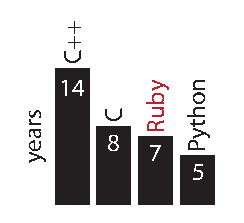
\includegraphics[width=2in]{programming-graph.pdf}%
\begin{tikzpicture}
\begin{axis}[ybar
			, symbolic x coords={C++, C, Ruby, Python, Matlab},
			, ylabel={years}
			, ylabel near ticks
			, ymajorgrids=true
			, axis on top
			, grid style={draw=white, line width=1pt}
			, major tick length=0pt
			, ymin=0
			, xtick=data
			, fill=black
			, fill opacity=1.0
			, draw=white
			, bar width=0.05\textwidth
			, nodes near coords
			, every node near coord/.append style={rotate=90, anchor=west, color=black}
			, width=2in
			, xmajorticks=false
			]
\addplot+[point meta=explicit symbolic,fill=black,draw=white] coordinates {
	(C++,21) [C\footnotesize{++}]
	(C,15) [C]
	(Ruby,10) [Ruby]
	(Python,11) [Python]
	(Matlab,3) [Matlab]
};
\end{axis}
\end{tikzpicture}
\vspace{-15pt}%
\end{wrapfigure}%

\mhead{Coding \newline Proficiencies}%
%
%\emph{Strong}\ 
\textsc{c},
\Cpp,
Ruby,
Python,
\LaTeX,
\textsc{gnu} Octave / Matlab

\medskip
\emph{Familiar}\ 
Java, \textsc{sql}, shell scripting, Agile, Go

\medskip
\emph{Forgotten}\
Perl, Fortran~95, Clojure, regular expressions

\medskip
\emph{Libraries}\ 
Orekit,
\textsc{cspice} (\textsc{jpl naif}),
\Cpp\ \textsc{stl} and Boost,
%\textsc{assimp},
%ImageMagick/\Magickpp,
%\textsc{atlas},
%\textsc{lapack},
%\textsc{blas},
%\textsc{gnu} Scientific Library,
Open\textsc{gl},
%\textsc{glm},
%Eigen,
$\varnothing$mq,
\textsc{Trick} simulator

\medskip
\emph{Contributions}\ 
Spiceypy, %$^\dagger$,
Point Cloud Library, %$^\dagger$,
\textsc{flann}, %,$^\dagger$ ($k$ nearest neighbors),
\textsc{Nm}atrix$^\dagger$ (Ruby linear algebra library),
Pyquat$^\dagger$ (Python attitude library),
\textsc{Glidar}$^\dagger$ (\textsc{3d lidar} simulator)
\\*
\medskip
%$^\dagger$\,{\footnotesize indicates code contributed to library}\hskip 1em
$^\dagger$\,{\footnotesize indicates primary authorship}

\medskip
\emph{Software}\
Copernicus, 
Satellite Toolkit (\textsc{stk}),
Git,
%Gnuplot,
%Emacs,
%Vim,
%Bash,
%Zsh,
\textsc{gcc},
Clang,
\textsc{gdb},
Valgrind,
\textsc{cm}ake,
Ubuntu,
Mac~\textsc{os\,x},
\textsc{gnu} Radio
\bigskip

\mhead{Education}%
\textbf{The University of Texas at Austin,} Austin, Texas \newline
\emph{Doctor of Philosophy, Cell \& Molecular Biology (Bioinformatics)}\rdate{2007--2013}
\begin{itemize*}
  \item National Science Foundation Fellow (2009--2012), \href{http://cssb.utexas.edu/}{Center for Systems \& Synthetic Biology} % 3.7646 GPA
% \item Dissertation: \href{https://www.dropbox.com/s/87v8j47mxo0afgj/diss.pdf}{Predicting gene--phenotype associations in humans and other species from orthologous and paralogous phenotypes}
  \item Advisor: Dr.~Edward~M.~Marcotte
\end{itemize*}

\medskip
\textbf{Virginia Polytechnic Institute \& State University,} Blacksburg, Virginia \newline
\emph{Bachelor of Science, Computer Science}, magna cum laude \rdate{2002--2007}
\begin{itemize*}
  %\item Graduated \emph{magna cum laude} % 3.66 GPA
  \item Minors in Mathematics, Philosophy, and Russian
\end{itemize*}
%
\bigskip
\mhead{Professional \newline Appointments}%
\vskip -1em
\textbf{Charm Industrial,} San Francisco, California \newline
\emph{Senior control systems engineer} \rdate{\textsc{oct}~2022--\textsc{may}~2023}
\begin{itemize*}
    \item Designed, implemented, and hardware tested custom process automation framework (finite state automata and various \textsc{pid} controllers) for use with programmable logic controllers
    \item Wrote plant models for chemical engineering processes in fast pyrolysis-based carbon sequestration
\end{itemize*}
%
\medskip
\textbf{Masten Space Systems,} Mojave, California \newline
\emph{\textsc{gn\&c} engineer, 6-\textsc{dof} (contractor)} \rdate{\textsc{jul}~2021--\textsc{jun}~2022}
\begin{itemize*}
%   \item Derived, designed, and prototyped \textsc{ekf} for \textsc{xl}-1 lunar lander
%   \item Designed flight manager for high-level planning of \textsc{gn\&c} activities
   \item Derived, designed, and prototyped extended Kalman filter for integrating sensor data into time series least squares model, including attitude
   \item Designed state machine for automating spacecraft behaviors
   \item Advised organization on diversity, equity, and inclusion as part of \textsc{de\&i} council
\end{itemize*}
%
\medskip
\textbf{Charismatic Metafauna by Majorelle Arts,} Oakland, California \newline
\emph{Sound Design Team Lead} \rdate{2021--2022}
\begin{itemize*}
   \item Wrote engineering requirements / system specifications for sound design for a large-scale interactive art project (\$30\textsc{k} budget, ~20 volunteers)
   \item Coordinating activities of sound design team and interfacing with interactivity team to fulfill engineering requirements
\end{itemize*}
%
\medskip
\textbf{Numina Studios / Nocturne-X,} Oakland, California \newline
\emph{Electronics Assembly (contractor)} \rdate{\textsc{sep}--\textsc{oct}~2021}
%\begin{itemize*}
%   \item Soldering and electronics assembly for a large-budget interactive art experience at Gray Area in San Francisco for three months beginning October~2021
%\end{itemize*}
%
%\medskip
%\textbf{Metalunar, \textsc{\textbf{llc}}}, Boulder, Colorado / \textbf{Translunar, \textsc{\textbf{llc}}}, Berkeley, California \newline
%\emph{Co-founder} \rdate{\textsc{apr}~2020--\textsc{present}}
%\begin{itemize*}
%  \item Systems engineering: \textsc{gn\&c} systems, optical navigation, and interplanetary radios (LunaNet)
%  \item Business models (system requirements, budget, timeline, market analysis) 
%  \item Proposal writing
%\end{itemize*}

\medskip
\textbf{Open Lunar Foundation,} San Francisco, California \newline
%\begin{itemize*}
%  \item Worked with small team to develop strategy for a space industry non-profit focused on lunar settlement
%  \item Analyzed 
%  \item Created business plans, engineering schedules, and financial models for various for-profit interventions
%\end{itemize*}
\emph{Senior Researcher} \rdate{\textsc{mar}--\textsc{jul}~2021} \\
\emph{Director of Engineering Research \& Strategy} \rdate{\textsc{jul}~2020--\textsc{mar}~2021} \\
\emph{Guidance, Navigation, \& Control} \rdate{\textsc{oct}~2019--\textsc{apr}~2020}
\begin{itemize*}
  \item Managed a research fellow to create business plans, engineering schedules, and financial models for various for-profit and non-profit interventions
  \item Engineering designs and analyses
  %\item Designs and analyses: \textsc{ekf}, \textsc{bls} for orbit determination, sensors, trajectory
%  \item Proposed a pipeline for generating vision-based navigation databases; studied positioning, navigation, and timing architectures %Submitted export control advisory opinion request to DDTC.
  \item Space policy: multilateral arms control treaties, export control policy, open source, electronic frontiers
  \item Systems engineering: \textsc{gn\&c} systems, optical navigation, and interplanetary radios (LunaNet)
\end{itemize*}

\medskip
\textbf{Intuitive Machines,} Houston, Texas \newline
\emph{Senior Development Engineer} \rdate{\textsc{jun}~2015--\textsc{sep}~2019} % June 22 - Sep 27
\begin{itemize*}
  \item Trajectory design \& optimization; lunar mission design \& analysis (\textsc{nova-c})%; sensor model simulations%; measurement model derivations; reaction control system trade study
  \item Documented and validated extended Kalman filter (Moon Express \textsc{mx}-1)
  \item \textsc{iss} rendezvous/berthing plan, preliminary \textsc{gn\&c} design (Axiom) %; prototyped quaternion feedback (eigenaxis) control algorithm; implemented candidate optimal group jet selection algorithm; performed control authority analysis
  \item State estimation (\textsc{bls}, \textsc{ekf}, complementary) for drilling systems
%  \item Performed observability analysis of gimbaled single-axis rate-integrating gyroscope for gyrocompassing; built batch least squares calibration and estimation strategy in \textsc{Matlab}
%  \item Mission hardware and software support, wrote measurement models and extended Kalman filter for
  \item \textsc{gps}-denied navigation and gravimetry (Doppler \textsc{lidar})
%  \item Cislunar navigation architectures: dilution of precision
%  \item Open source Python attitude and unit quaternion library (pyquat)
%  \item Responsible for universal navigation filter in \textsc{im}'s universal flight software, to be flown on a deorbiter (Terrestrial Return Vehicle, or \textsc{trv}) and Moon Express' moon lander; documented and re-derived filter; wrote and validated sensor models in \textsc{nasa} \textsc{trick} physics simulator
  \item Wrote engineering requirements for payloads, including for molecular biology in microgravity
% 
%  \item Designed and implemented multiple dual-state extended Kalman filters and complementary filters for aircraft, spacecraft, and drilling systems
%  \item Performed error budget analysis and designed and prototyped \textsc{ekf} for gravimetry and \textsc{gps}-denied planetary navigation
\end{itemize*}

\bigskip
\mhead{Academic \newline Appointments}%
\textbf{Applied Space Exploration Laboratory,} West Virginia University \newline
\emph{Post-doctoral Fellow --- Aerospace Engineer} \rdate{\textsc{jan}~2014--\textsc{jun}~2015}
\begin{itemize*}
  \item \textsc{Lidar}-based \textsc{6\,dof} pose initialization strategy for non-cooperative rendezvous; derived/implemented dual inertial state \textsc{ekf} (satellite servicing)% with asynchronous measurement updates
  \item Open source Open\textsc{gl}-based \textsc{3d} sensor simulator, \textsc{Glidar}
  \item Remote sensing technologies for resource surveying and utilization
  \item Mentored and collaborated with grad students and an undergraduate
\end{itemize*}

\medskip
\textbf{Center for Systems \& Synthetic Biology,} The University of Texas at Austin\newline
\emph{National Science Foundation Fellow; Graduate Research Assistant}  \rdate{2007--2014}
\begin{itemize*}
  \item Pipelines and automation for large datasets
  \item Researched, designed, and wrote statistical software for searching for genes under various types of selection (positive, purifying, relaxed)
  \item Invalidated a hypothesis about \textsc{hiv} reservoirs using viral evolution simulation
  \item Designed scheme for re-engineering cellular metabolism in \textit{E.~coli}, and partially implemented it (wet lab)
  \item Some experience with mass spectrometry-based proteomics
\end{itemize*}

\medskip
\textbf{Dept. of Chemistry \& Biochemistry,} The University of Texas at Austin\newline
\emph{Graduate Teaching Assistant} \rdate{2008, 2013}
\begin{itemize*}
%  \item Served as \textsc{ta} for Biochemistry, Introduction to Bioinformatics (graduate level), and Chemistry for non-science majors
  \item Rewrote curriculum in Python (previously in Perl)
\end{itemize*}
%\newpage
\bigskip
\mhead{Patents}%
\par\vspace{-\baselineskip}Marcotte, E.M.; McGary, K.; Wallingford, J.; Park, T.J.; \textbf{Woods,~J.O.}; Cha,~H.J. 12 August 2012. Orthologous phenotypes and non-obvious human disease models. \textit{U.S.\ Patent Application Publication 2012/0215458 A1}.

\bigskip
%\newpage
\mhead{Articles}%
\par\vspace{-\baselineskip}%\textit{List of non-aerospace articles authored available upon request.}
%\medskip
\par\textbf{Woods, J.O.}; Christian, J.A. 2016. \textsc{Lidar}-based relative navigation with respect to non-cooperative objects. \textit{Acta Astronautica 126}: pp.\ 298--311.

\medskip
\par\textbf{Woods, J.O.}; Christian, J.A. 2016. \textsc{Glidar}: An OpenGL-based, real-time, and open source 3\textsc{d} sensor simulator for testing computer vision algorithms. \textit{Journal of Imaging 2}(1).

\medskip
\par\textbf{Woods, J.O.}; Tien, M.Z.; Marcotte, E.M. April 2015. Interrogating conserved elements of diseases using Boolean combinations of orthologous phenotypes. \textit{BioR$\chi$iv}.

\medskip
\par\textbf{Woods, J.O.}; Singh-Blom, U.M.; Laurent, J.M.; McGary, K.L.; Marcotte, E.M. January 2013. Prediction of gene--phenotype associations in humans, mice, and plants using phenologs. \textit{BMC Bioinformatics 14}: p.\ 203.

\medskip
\par Singh-Blom, U.M.; Natarajan, N.; Tewari, A.; \textbf{Woods, J.O.}; Dhillon, I.S.; Marcotte, E.M. January 2013. Prediction and validation of gene--disease associations using methods inspired by social network analyses. \textit{PLoS One 8}(5): e58977.

\medskip
\par McGary, K.L.; Park, T.J.; \textbf{Woods, J.O.}; Cha, H.J.; Wallingford, J.B.; Marcotte, E.M. April 2010. Systematic discovery of nonobvious human disease models through orthologous phenotypes. \textit{Proceedings of the National Academy of Sciences of the United States of America 107}(14): pp.\ 6544--9.

\medskip
\par Brennan, T.P.; \textbf{Woods, J.O.}; Sedaghat, A.R.; Siliciano, J.D.; Siliciano, R.F.; Wilke, C.O. September 2009. Analysis of human immunodeficiency virus type 1 viremia and provirus in resting $\textsc{cd4}^{+}$ \textsc{t} cells reveals a novel source of residual viremia in patients on antiretroviral therapy. \textit{Journal of Virology 83}(17): pp.\ 8470--81.

%\newpage
\bigskip
\mhead{Conference \newline Proceedings}%
\par\vspace{-\baselineskip}\textbf{Woods, J.O.}; Christian, J.A.; Evans, T. February 2015. A \textsc{6-dof} pose initialization strategy for \textsc{lidar}-based non-cooperative navigation. In \textit{38th Annual Guidance \& Control Conference}, Breckenridge, CO.

\medskip
Sell, J.L.; Rhodes, A.; \textbf{Woods, J.O.}; Christian, J.A.; Evans, T. 2014. Pose performance of LIDAR-based navigation for satellite servicing. In \textit{AIAA/AAS Astrodynamics Specialist Conference}, San Diego, CA.

\bigskip
\mhead{Posters}%
\par\vspace{-\baselineskip}\textbf{Woods, J.O.}; Singh-Blom, U.M.; Laurent, J.; McGary, K.L.; Marcotte, E.M. 20--25 February 2012. In \textit{Complex Traits: Genomics and Computational Approaches}, Keystone Symposia, Breckenridge, CO.

\medskip
\par \textbf{Woods, J.O.}; Singh-Blom, U.M.; McGary, K.L.; Marcotte, E.M. 13--16 November 2010. In \textit{From Functional Genomics to Systems Biology},  EMBL Heidelberg, Heidelberg, Germany.

\bigskip
\mhead{Technical \newline Reports}%
\par\vspace{-\baselineskip}\textit{Some internal technical report titles have been changed for external clarity or to maintain client confidentiality.}

\medskip
\par\textbf{Woods, J.O.} 2021. An engineer's history of US and multilateral export controls. \textit{OLF--ENG--2021--01}, Open Lunar Foundation, San Francisco, CA.

\medskip
\par\textbf{Woods, J.O.} 2020. Concepts in lunar positioning, navigation, and timing. \textit{OLF--GNC--2020--01}, Open Lunar Foundation, San Francisco, CA.

\medskip
\par\textbf{Woods, J.O.} 2019. Navigation filter design towards a lunar lander. \textit{OLF--GNC--2019--02}, Open Lunar Foundation, San Francisco, CA. \textit{Work in progress, ceased and published early due to pandemic.} \href{https://github.com/openlunar/navmemos/raw/master/filter/filter.pdf}{github.com/openlunar/navmemos/ raw/master/filter/filter.pdf}

\medskip
\par\textbf{Woods, J.O.} 2019. Two-way range and range-rate observables in a sequential filter. \textit{OLF--GNC--2019--01}, Open Lunar Foundation, San Francisco, CA. \href{https://github.com/openlunar/navmemos/raw/master/radiometric/memo.pdf}{github.com/openlunar/navmemos/raw/master/radiometric/memo.pdf}

\medskip
\par\textbf{Woods, J.O.} 2018. Observability and sensitivity analyses for attitude estimation using a gimballed gyroscope. \textit{IM--TM--2018--04}.

\medskip
\par \textbf{Woods, J.O.} 2018. Position and velocity variance growth during dead reckoning of a drill. \textit{IM--TM--2018--02}.

\medskip
\par \textbf{Woods, J.O.} 2018. Derivation of the Doppler \textsc{lidar} measurement model in the inertial and topocentric frames. \textit{IM--TM--2018--01}.

\medskip
\par Crain, T.C.; \textbf{Woods, J.O.}; Baine, M.; Moore, J.; Getchius, J.; Ronalds, A.; Stewart, S. 2018. Cislunar navigation architecture study. \textit{IMDM--9}.

\medskip
\par \textbf{Woods, J.O.} 2017. A dual \textsc{marg} complementary filter for attitude state estimation while drilling. \textit{IM--TM--2017--04}.

\medskip
\par \textbf{Woods, J.O.}; Christian, J.A. 2014. A real-time, software-based \textsc{3d} sensor simulator. ASEL Technical Memorandum: \textit{ASEL--14--005}.

\medskip
\par Sell, J.; Rhodes, A.; \textbf{Woods, J.}; Christian, J.A. 2014. Theoretical foundations of pose estimation and covariance computation for non-cooperative relative navigation. ASEL Technical Memorandum: \textit{ASEL--14--001}.

\medskip
\par Natarajan, N.; Singh-Blom, U.M.; Tewari, A.; \textbf{Woods, J.O.}; Dhillon, I.S.; Marcotte, E.M. 2011. Predicting gene--disease associations using multiple species data. UTCS Technical Report: \textit{TR--11--37}.

\bigskip
%\newpage
\mhead{Selected \\ Honors \& \newline Awards}%
Burning Man Honorarium: \textit{Charismatic Metafauna}				\rdate{2022}\newline
Masten Space Systems: Diversity, Equity, and Inclusion Council member \rdate{2022}\newline
%Paul Harris Fellowship                                              \rdate{2018}\newline
%Necklace Factory / Burning Man Art Award                            \rdate{2016}\newline
White House Champion of Change				\rdate{2014}\newline
National Science Foundation Graduate Research Fellowship			\rdate{2009--2012}\newline
``Best of Austin'' Award: Best Activist	(\emph{The Austin Chronicle})							\rdate{2011}\newline
Scholar, Netroots Nation											\rdate{2011}\newline
Initiate, Friar Society (University of Texas at Austin)				\rdate{2010}\newline
Graduate School Recruitment Fellowship (University of Texas at Austin) \rdate{2007}\newline
Black Belt, Tae Kwon Do (Chung Do Kwan)								\rdate{2006}\newline
Member, Hillcrest Honors Community (Virginia Tech)				\rdate{2003--2007}\newline
Inductee, $\Upsilon\Pi\mathrm{E}$ (Virginia Tech)					\rdate{2006}\newline
Gilbert \& Lucille Seay Scholarship (Virginia Tech)					\rdate{2005}\newline
National Merit Scholarship											\rdate{2002}%\newline

\bigskip
\mhead{Community Contributions}
\vskip -1em
\textbf{Lunar Surface Innovation Consortium}\rdate{2021--\textsc{present}}\newline
\emph{Communications Subgroup Lead} \rdate{2021--2022}

\medskip
\textbf{Black Rock Rangers}\rdate{2018--\textsc{present}}\newline
\emph{Green Dot} \rdate{2019--\textsc{present}}

\medskip
\textbf{Ruby Science Foundation (SciRuby)} \newline %The Ruby Science Foundation: The SciRuby Project}\newline
\emph{Director \& Co-Founder} \rdate{2012--2018}

%\medskip
%\textbf{Austin Swing Syndicate}\newline
%\emph{At-Large Board Member, Secretary} \rdate{2012--2014}%\newline%
%
\medskip
\textbf{Texas Gun Sense}\newline
\emph{Co-founder, Advisory Board Member} \rdate{2013--\textsc{present}}%\newline

%\bigskip
%\mhead{Media}%
%\par\vspace{-\baselineskip}\textit{Media appearances available upon request.}
\bigskip
\mhead{Activities \& \newline Interests}%
dance (lindy hop and ballet),
music,
roller skating,
circus arts,
space exploration,
large-scale interactive art,
immersive theatre

\bigskip
%French, German, Mandarin (smattering)
%\newpage
\mhead{Foreign\newline Languages}%
English (native tongue), 
Spanish (conversational), 
Russian (needs refreshing)
%German,
%Mandarin

\bigskip
\mhead{Other Skills}%
Metal fabrication and \textsc{mig} welding, fiberglass/resin casting, \textsc{fema~ics}-100 certification

\bigskip
\mhead{References}%
Chris~Hadfield\rdate{\href{mailto:chris@chrishadfield.ca}{chris@chrishadfield.ca}}\newline
Chair, Open Lunar Foundation; Commander, \textsc{csa} and \textsc{nasa}

\medskip
John~Christian\rdate{\href{mailto:john.christian@mail.wvu.edu}{john.christian@mail.wvu.edu}}\newline
Asst.\ Professor of Aerospace Engineering, Rensselaer Polytechnic Institute

\medskip
Tim~Crain\rdate{\href{mailto:tim@intuitivemachines.com}{tim@intuitivemachines.com}}\newline
Vice President of Research and Development, Intuitive Machines

\medskip
Amanda~Acevedo\rdate{\href{mailto:amanda.acevedo@vedosystems.com}{amanda.acevedo@vedosystems.com}}\newline
President, Vedo Systems; formerly Project Manager, Intuitive Machines

\medskip
Ben~Howard\rdate{\href{mailto:ben@openlunar.org}{ben@openlunar.org}}\newline
Chief Engineer, Open Lunar Foundation; Chief Spacecraft Architect, Planet

\medskip
Eva Pettinato\rdate{\href{mailto:eva.pettinato@gmail.com}{eva.pettinato@gmail.com}}\newline
Lead Guidance, Navigation, and Control Engineer, Masten Space Systems

\medskip
Edward~Marcotte\rdate{\href{mailto:marcotte@icmb.utexas.edu}{marcotte@icmb.utexas.edu}\hskip 0.5cm\href{tel:512-471-5435}{512-471-5435}}\newline
Professor of Chemistry \& Biochemistry, The University of Texas at Austin
\end{document}